%%%%%%%%%%%%%%%%%%%%%%%%%%%%%%%%%%%%%%%%%
% baposter Landscape Poster
% LaTeX Template
% Version 1.0 (11/06/13)
%
% baposter Class Created by:
% Brian Amberg (baposter@brian-amberg.de)
%
% This template has been downloaded from:
% http://www.LaTeXTemplates.com
%
% License:
% CC BY-NC-SA 3.0 (http://creativecommons.org/licenses/by-nc-sa/3.0/)
%
%%%%%%%%%%%%%%%%%%%%%%%%%%%%%%%%%%%%%%%%%

%----------------------------------------------------------------------------------------
%	PACKAGES AND OTHER DOCUMENT CONFIGURATIONS
%----------------------------------------------------------------------------------------

\documentclass[landscape,a0paper,fontscale=0.285]{baposter} % Adjust the font scale/size here

\usepackage{graphicx} % Required for including images
\graphicspath{{figures/}} % Directory in which figures are stored

\usepackage{amsmath} % For typesetting math
\usepackage{amssymb} % Adds new symbols to be used in math mode

\usepackage{booktabs} % Top and bottom rules for tables
\usepackage{enumitem} % Used to reduce itemize/enumerate spacing
\usepackage{palatino} % Use the Palatino font
\usepackage[font=small,labelfont=bf]{caption} % Required for specifying captions to tables and figures

\usepackage{multicol} % Required for multiple columns
\setlength{\columnsep}{1.5em} % Slightly increase the space between columns
\setlength{\columnseprule}{0mm} % No horizontal rule between columns

\usepackage{tikz} % Required for flow chart
\usetikzlibrary{shapes,arrows} % Tikz libraries required for the flow chart in the template

\newcommand{\compresslist}{ % Define a command to reduce spacing within itemize/enumerate environments, this is used right after \begin{itemize} or \begin{enumerate}
\setlength{\itemsep}{1pt}
\setlength{\parskip}{0pt}
\setlength{\parsep}{0pt}
}

\definecolor{lightblue}{rgb}{0.145,0.6666,1} % Defines the color used for content box headers

\begin{document}

\begin{poster}
{
headerborder=closed, % Adds a border around the header of content boxes
colspacing=1em, % Column spacing
bgColorOne=white, % Background color for the gradient on the left side of the poster
bgColorTwo=white, % Background color for the gradient on the right side of the poster
borderColor=lightblue, % Border color
headerColorOne=black, % Background color for the header in the content boxes (left side)
headerColorTwo=lightblue, % Background color for the header in the content boxes (right side)
headerFontColor=white, % Text color for the header text in the content boxes
boxColorOne=white, % Background color of the content boxes
textborder=roundedleft, % Format of the border around content boxes, can be: none, bars, coils, triangles, rectangle, rounded, roundedsmall, roundedright or faded
eyecatcher=true, % Set to false for ignoring the left logo in the title and move the title left
headerheight=0.1\textheight, % Height of the header
headershape=roundedright, % Specify the rounded corner in the content box headers, can be: rectangle, small-rounded, roundedright, roundedleft or rounded
headerfont=\Large\bf\textsc, % Large, bold and sans serif font in the headers of content boxes
%textfont={\setlength{\parindent}{1.5em}}, % Uncomment for paragraph indentation
linewidth=2pt % Width of the border lines around content boxes
}
%----------------------------------------------------------------------------------------
%	TITLE SECTION 
%----------------------------------------------------------------------------------------
%
{
\includegraphics[height=8em]{cyi.png}} % First university/lab logo on the left
{\bf\textsc{\LARGE{Enabling Performance-Portability of Full Wavefield Migration \newline for seismic tomography}}\vspace{0.5em}} % Poster title
{ Andreas Hadjigeorgiou, \hspace{11pt} The Cyprus Institute, CaSToRC} % Author names and institution
{
\includegraphics[height=6em]{delphi.png}} % Second university/lab logo on the right

%----------------------------------------------------------------------------------------
%	INTRODUCTION
%----------------------------------------------------------------------------------------

\headerbox{Introduction}{name=introduction,column=0,row=0,span=2}{
    
\begin{multicols}{2}
    Seismic migration is the process of geometrically locating the seismic events to the positions 
    in space (or time) where they occurred. In principle, the migration process relies on modelling 
    wavefields that propagate through the subsurface. Accurate migration requires the knowledge of 
    the subsurface proporties, which is at the same time the subject matter; this makes it an inverse problem. 
    Full Wavefield Migration (FWM) is an iterative migration scheme that optimizes subsurface 
    delineation by employing in the imaging process \textit{primary} as well as \textit{higher-order} scattering 
    effects. However, this comes at higher computational cost. In realistic seismic surveys 
    the amount of data that needs to be processed is in the order of Petabytes. On top of this, 
    the iterative process introduced by the FWM scheme makes the computational complexity of the 
    process such high, that supercomputing level resources are needed in order to make 
    applications practical.
    
    \begin{center}
        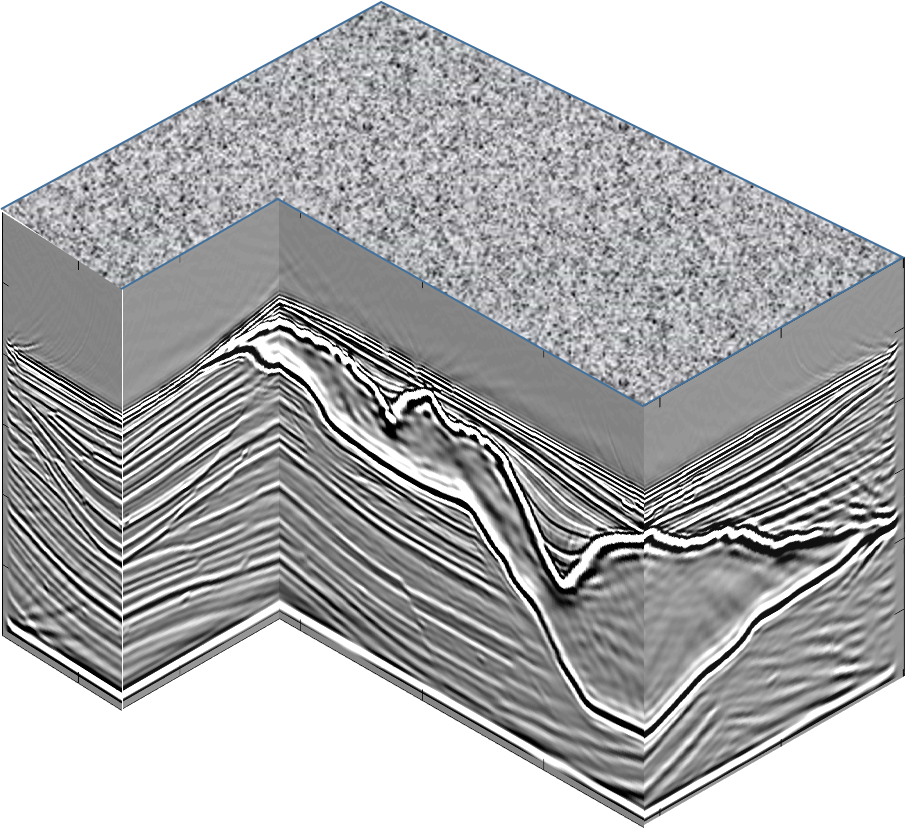
\includegraphics[width=7.0cm,height=6cm]{figures/3D_image.png}
    \end{center}

    The evolution in HPC from parallel processing on single-core to many-core processing units 
    of different architectures such as CPUs, GPUs, FPGAs, and other emerging hardware, 
    makes portability - without performance loss - a real challenge!%; most often a trade-off!

\end{multicols}

}

%----------------------------------------------------------------------------------------
%	OBJECTIVES
%----------------------------------------------------------------------------------------

\headerbox{Objectives}{name=objectives,column=0,row=1,span=2,below=introduction}{

\begin{itemize}
 \item Optimize the wavefield modelling engine, which is the most computationally complex operation in FWM, for CPU and GPU architectures using platform-specific implementations.

 \item Develop platform-specific routines that provide additional essential functionalities for FWM.

 \item Develop an abstraction layer in C++ that makes these platform-specific implementations accessesible through a common interface.

 \item Develop a set of containers (classes) and routines (funtions) that adhere to the C++ abstraction layer,
 to ease the development of algorithms.

 \item Using the C++ abstraction layer develop performance-portable FWM for seismic imaging.
\end{itemize}

\vspace{0.3em} % When there are two boxes, some whitespace may need to be added if the one on the right has more content
}

%----------------------------------------------------------------------------------------
%	CODE DESIGN
%----------------------------------------------------------------------------------------

\headerbox{Code design}{name=code,column=2,span=2,row=0}{
    \begin{multicols}{2}
        \vspace{1em}
        \begin{center}
            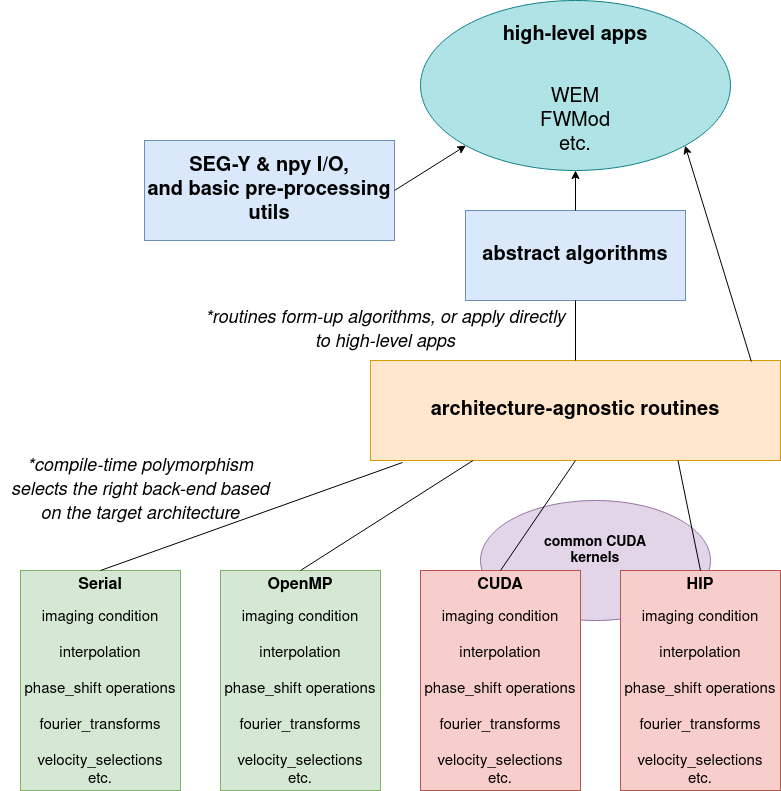
\includegraphics[width=8cm]{CODE_design_drawio.png}
        \end{center}

        \textbf{Portability-approach}: Different platform-specific back-end implementations adhere 
        to one abstract interface, enabling portability across a range of CPU/GPU computer 
        architectures for the high-level applications that are built on top of.
        \smallskip

        \textbf{Performance-approach}: Use the right programming model for each target architecture.

        \begin{itemize}
            \item Develop the \textit{Serial} implementation for reference.
            \item Use OpenMP threads for CPU parallelism.
            \item Use CUDA for acceleration on Nvidia GPU.
            \item Use HIP layer to port CUDA on AMD GPUs.
        \end{itemize}
    \end{multicols}
}

%----------------------------------------------------------------------------------------
%	REFERENCES
%----------------------------------------------------------------------------------------

\headerbox{References}{name=references,column=0,span=2,above=bottom,below=objectives}{

\renewcommand{\section}[2]{\vskip 0.05em} % Get rid of the default "References" section title
% \nocite{*} % Insert publications even if they are not cited in the poster
\small{ % Reduce the font size in this block
\bibliographystyle{unsrt}
\bibliography{sample} % Use sample.bib as the bibliography file
}
}

%----------------------------------------------------------------------------------------
%	CONTACT INFORMATION - FEEDBACK WOULD BE APPRECIATED
%----------------------------------------------------------------------------------------

\headerbox{Contact Information - Any feedback is welcome!!!}{name=contact,column=2,span=2,above=bottom}{
    \textbf{Personal page}: https://ahadji05.github.io, \
    \textbf{Email}: a.hadjigeorgiou@cyi.ac.cy, \ \textbf{Phone}: +357 99839383
}

%----------------------------------------------------------------------------------------
%	PRELIMINARY RESULTS
%----------------------------------------------------------------------------------------

\headerbox{Preliminary results}{name=results,column=2,span=1,below=code,above=contact}{ % This block is as tall as the references block

    \textbf{So far}: Effectively ported the wavefield modelling engine [1] on Intel, 
    AMD CPUs, and Nvidia, AMD GPUs. On top of the modelling engine we have developed 
    one-iteration migration algorithms like Wave-Equation Migration [2], and currently 
    working on more sophisticated iterative migration algorithms like FWM [3,4].

    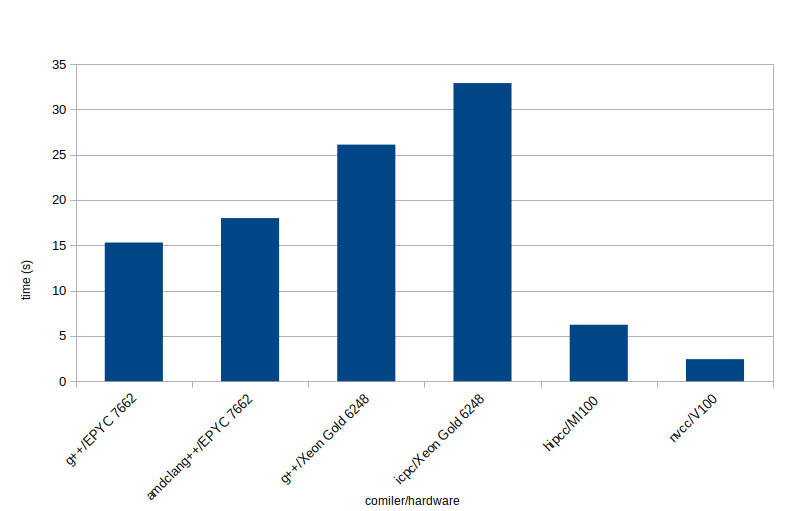
\includegraphics[width=7.0cm]{perfport.png}

    \textbf{Next}: MPI+X for distributed parallelism!
}

%----------------------------------------------------------------------------------------
%	REMARKS
%----------------------------------------------------------------------------------------

\headerbox{Remarks}{name=remarks,column=3,span=1,below=code,above=contact}{

    \begin{itemize}
        \item Using OpenMP and CUDA we enable portability of FWM to almost all available hardware 
        in todays supercomputers.
        \item The portability to HIP was generally trivial, including the \textit{hipFFT} library.
        \item To enable portability with this approach, that additional code-development effort was 
        30-40 \%.
        \item Unit-testing applies to architecture-agnostic routines level (\textit{see fig.});
        it was not necessary to write unit-tests explicitly for each implementation.
        %\item ...
    \end{itemize}
}

\end{poster}

\end{document}